\chapter{FUNDAMENTAÇÃO TEÓRICA}
\label{cap:fundamentacao-teorica}

  \section{Reincidência Criminal}
		
Reincidência criminal se resume em um agente egresso do sistema prisional que cometeu um novo crime depois do cumprimento da pena estabelecida por um crime anteriormente cometido e depois de 5 anos de transitado e julgado, não cabe mais recurso ao ato do crime anterior conforme... Porém a reincidência criminal pode ser definida de 6 maneiras distintas, segundo:

\begin{enumerate}
	\item Reincidência por auto culpa, que considera nova prática de crime declarada pelo mesmo indivíduo. 
	\item Reincidência policial, que é estabelecida por novo registro de crime do mesmo indivíduo na polícia. 
	\item Reincidência penal, que supõe o processamento penal do mesmo indivíduo por nova prática de crime. 
	\item Reincidência judicial, que envolve nova condenação do mesmo indivíduo por nova prática de crime. 
	\item Reincidência penitenciária, que ocorre quando há segundo ingresso na prisão do mesmo indivíduo por nova prática criminal.
	\item Reincidência jurídica, que é o segundo processamento do mesmo indivíduo por nova prática de crime do mesmo título do Código Penal.
\end{enumerate}		
		 
		
Existem diferentes abordagens segundo Julião (2009), Adorno e Bordini (1989) e Pinatel (1984) que sugerem diferenciar quatro tipos de reincidência: i) reincidência genérica, que ocorre quando há mais de um ato criminal, independentemente de condenação, ou mesmo autuação, em ambos os casos; ii) reincidência legal, que, segundo a nossa legislação, é a condenação judicial por novo crime até cinco anos após a extinção da pena anterior;	iii) reincidência penitenciária, quando um egresso retorna ao sistema penitenciário após uma pena ou por medida de segurança; iv) reincidência criminal, quando há mais de uma condenação, independentemente do prazo legal. Inclusive, a tentativa de mensurar a reincidência ganha diferentes contornos metodológicos, dependendo do tipo de conceito que se assume.
		
fizeram uma pesquisa em São Paulo onde avaliaram a magnitude da reincidência penitenciaria e conhecer e interpretar o perfil social dos reincidentes, e comparando-os com os não reincidentes. A pesquisa foi feita no período entre janeiro 1974 a dezembro de 1985, verificando se houve um retorno dos indivíduos ao sistema penitenciário ou cadeia publicas do estado de São Paulo e foi encontrada uma taxa de reincidência penitenciária de 46,03\%.
		
O estudo de Lemgruber (1989) foi realizado no Rio de Janeiro com a intenção de dimensionar a reincidência penitenciaria onde o estudo ocorreu no ano de 1988 pelo Departamento do Sistema Penal (Desipe) e o levantamento quantitativo dos totalizou 8.269 presos e 251 presas. Por meio deste resultados desta pesquisa obteve a taxa de reincidência de 30,7\%, sendo a referente aos homens de 31,3\% e a referente às mulheres de 26\%.
		
O estudo do Instituto de Pesquisa Econômica Aplicada (IPEA) em 2015, teve como objetivo apresentar um panorama da reincidência criminal no Brasil através da coleta de dados em algumas unidades da federação. A pesquisa tem por foco casos em que há condenações de um indivíduo em diferentes ações penais, que ocorrem por fatos diversos. O estudo foi realizado nos estados: Paraná, Minas Gerais, Rio de Janeiro, Alagoas e Pernambuco. E a pesquisa resultou na taxa de reincidência 24,4\%, com predominância nas idades de 18 a 24 anos, do sexo masculino e com cor branca e os não reincidentes são pardos e negros.

	\section{ANÁLISE DE SOBREVIVÊNCIA}
		
			
Análise de Sobrevivência ou Sobrevida é a área da estatística que mais cresceu na década de 80 e no final desta época os artigos mais citados foram de \citeonline{kaplan1958nonparametric} e \citeonline{cox1972regression} segundo \cite{colosimo2006analise}

Análise de Sobrevivência tem como variável resposta o tempo até a ocorrência de um evento de interesse. Denominado tempo de falha. A característica principal dos dados de sobrevivência é sua particularidade com censura, ou seja, em alguns dos indivíduos observados não chegou a ocorrer o acontecimento de interesse, tem apenas observação parcial da resposta. 

    \subsection{FALHA, CENSURA E TRUNCAMENTO}

O tempo de falha precisa ser bem definido para não haver ambiguidades, conforme \citeonline{cox1984analysis} existem três requisitos: a origem do tempo; a escala para medir e normalmente é tempo-relógio; e o evento de interesse.	

A censura não é nada mais que uma observação parcial de um dado de sobrevivência. Três tipos de censuras podem ser considerados em estudos de sobrevida, ou seja:

\begin{itemize}
	\item [i)] Censura do tipo I:
	\item [ii)] Censura do tipo II:
	\item [iii)] Censura aleatória:
\end{itemize}

Além dos tipos de censuras há os mecanismos de censura que são: censura à direita, que é o mais normal em estudos de sobrevivência; censura à esquerda; e censura intervalar.

Os dados de sobrevida são representados em geral pelo par $(t_i,\delta_i)$ para o i-ésimo indivíduo sob estudo, sendo $t_i$ o tempo de falha ou censura e $\delta_i$ a variável indicadora de falha ou censura. 

O que se observa do i-ésimo indivíduo é

\begin{equation*}
\delta_i
= \left\{\begin{array}{rll}
1, & \hbox{se} & T_i \leq C_i \\
0, & \hbox{se} & T_i > C_i
\end{array}\right.
\end{equation*}


Os dados mesmo censurados devem ser usados na análise estatística. De acordo com \citeonline{colosimo2006analise} há duas razões que justificam tal procedimento: \textit{i}) mesmo sendo incompletos, as observações fornecem informações sobre o tempo de vida dos indivíduos; \textit{ii}) omitindo as censuras nas análises estatísticas de interesse pode implicar conclusões viciadas.


		 \subsection{FUNÇÃO DE SOBREVIVÊNCIA}

O tempo de falha de um determinado indivíduo em uma população homogênea é representado pela variável aleatória contínua não-negativa $T$. Define-se a função de sobrevivência de uma observação não falhar até um instante $t$, ou seja, a probabilidade dessa observação sobreviver ao tempo $t$. Em termos probabilísticos é representado como:

\begin{equation}\label{eq:survival-function}
	S(t) = P(T \geq t)
\end{equation},

\noindent que é uma função monótona, não crescente e contínua tendo as seguintes propriedades:

1. $S(0) = 1$;

2. $S(\infty) = \displaystyle{\lim_{t \to \infty}}S(t) = 0$

Outro conceito importante em consequência da função anterior é a função de distribuição acumulada que é definida como a probabilidade de uma observação não sobreviver ao tempo t, isto é, $F(t) = 1-S(t)$.

A função densidade de probabilidade $f(t)$ é definida como menos a derivada da função de sobrevivência:

\begin{equation}\label{eq:density-function-survival}
	f(t) = -\dfrac{\partial}{\partial t}S(t), \ \ t > 0.
\end{equation}

A interpretação dessa definição é que, para suficientemente pequeno $\Delta t$, a seguinte aproximação está próxima do valor verdadeiro:

\begin{equation}\label{eq:aprox-function}
	P(t \leq T < t + \Delta t) \approx \Delta t f(t)
\end{equation}

A figura mostra um intervalo bem pequeno $(t,t+s]$ tendo $s$ como termo infinitesimal. A probabilidade de uma observação contido nesse intervalo é bem aproximado por uma área de um retângulo com lados $s$ e $f(t)$. A definição matemática formal como limite é dada pela equação.

\begin{figure}[h!]
	\centering
		\caption{Interpretação da função de densidade $f$.}
			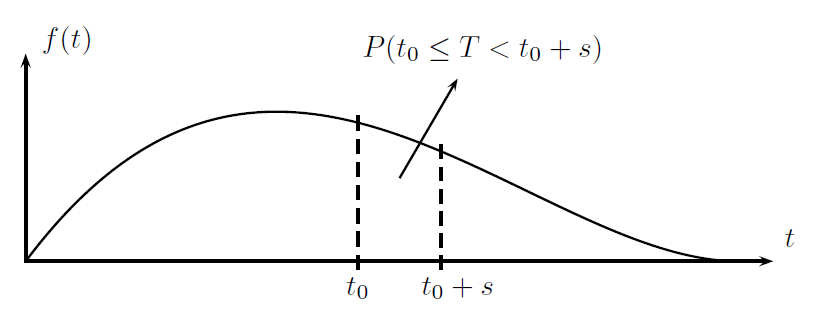
\includegraphics[scale=0.45]{img/fig1} \\
		Fonte: Douglas Vinícius
	\label{fig:figura2}
\end{figure}

\begin{equation}\label{eq:lim-survival}
	f(t) = \displaystyle{\lim_{\Delta t \to \infty}} \frac{P(t \leq T < t + \Delta t)}{\Delta t}
\end{equation}

		  \subsection{FUNÇÃO DE TAXA DE FALHA}

Podemos expressar a probabilidade da falha ocorrer em um intervalo de tempo $[t_1,t_2)$ em termos da função de sobrevivência como:

$$
S(t_1) - S(t_2).
$$

A taxa de falha em $[t_1,t_2]$ é definida como a probabilidade de que a falha ocorra neste intervalo, dado que não ocorreu antes de $t_1$, divida pelo comprimento do intervalo. Tendo como a taxa de falha de $[t_1,t_2)$ é representada por:

\begin{equation}\label{eq:taxa-de-falha}
	\frac{S(t_1) - S(t_2)}{(t_2 - t_1) \ S(t_1)}
\end{equation}

Em âmbito geral e redefinindo o intervalo como $[t, t + \Delta t)$, a expressão atribui-se da seguinte forma:

\begin{equation}\label{taxa-de-falha1}
	\lambda(t) = \frac{S(t) - S(t + \Delta t)}{\Delta t \ S(t)}
\end{equation}

A função $\lambda$(t) --- conhecida como função de risco (\textit{hazard function}), taxa instantânea de falha, taxa de falha ou força de mortalidade ---  é a taxa instantânea no tempo $t$ condicionado a sobrevivido até o tempo t. As taxas de falha são números positivos e sem limite superior. A utilidade da função de taxa de falha é ter uma descrição da distribuição e a forma que muda em relação ao tempo de vida dos indivíduos. 

A função de taxa de falha de $T$ é definida como:

\begin{equation}\label{hazard-function}
	\lambda(t) = \displaystyle{\lim_{\Delta t \to 0}} \frac{P(t \leq T < t + \Delta t | T \geq t)}{\Delta t }
\end{equation}

\noindent que satisfaz as seguintes propriedades: 

\begin{enumerate}
	\item $\lambda(t) \geq 0$;
	\item $\int_{0}^{\infty} \lambda(t) dt = \infty$.
\end{enumerate}



\begin{figure}[h!]
	\centering
	\caption{Monotonia da Função de Risco.}
	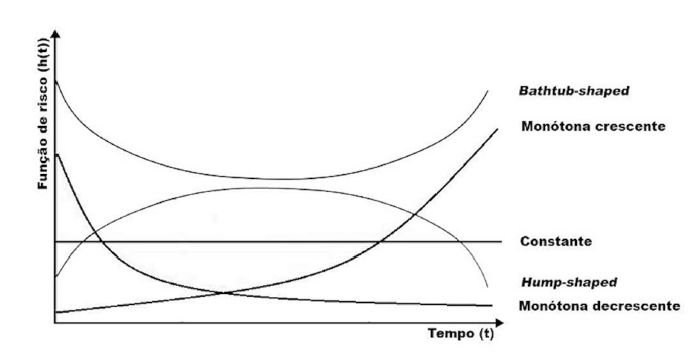
\includegraphics[scale=0.65]{img/fig3} \\
	Fonte: 
	\label{fig:figura3}
\end{figure}

		  \subsection{FUNÇÃO DE TAXA DE FALHA ACUMULADA}
			
A função de taxa de falha acumulada como o próprio nome já diz, fornece a taxa de falha acumulada, definida por:

\begin{equation}\label{eq:falha-acumulada}
	\Lambda(t) = \int_{0}^{t}\lambda(u)du
\end{equation},

\noindent isto é, mede 
			
      \subsection{TEMPO MÉDIO E VIDA MÉDIA RESIDUAL}

O Tempo Médio de vida é obtido pela função:

\begin{equation}\label{eq:tm}
	t_m = \int_{0}^{\infty} S(t)dt.
\end{equation}

Outra quantidade que mede a vida média restante de algum indivíduo observado com tempo t e chamada de Vida Média Residual é definida como:

\begin{equation}\label{eq:tm-vmr}
	vmr(t) = \frac{\int_{t}^{\infty}(u - t)f(u)du}{S(t)} = \frac{\int_{t}^{\infty}S(u)du}{S(t)}
\end{equation}

\noindent sendo $f(.)$ a função densidade de $T$.

Essas funções há relações importantes entre elas. Por exemplo, conhecendo $S(t)$ implica no conhecimentos das demais: $F(t)$, $f(t)$, $\lambda(t)$ e $\Lambda(t)$. Estas relações estão demonstradas no anexo A.

    \subsection{ESTIMADORES KAPLAN-MEIER}
      
      	\subsubsection{COMPARAÇÃO DE CURVAS DE SOBREVIVÊNCIA}
    
    \subsection{MODELO DE REGRESSÃO DE COX}
    
    	\subsubsection{ADEQUAÇÃO DO MODELO}
